\chapter{Data analysis}
\label{cap:data_analysis}

\section{Common procedures}
%\begin{itemize}
%\item Pedestal subtraction
%\item Common mode subtraction
%\item Gain equalisation
%\item Dismiss the low-end signal
%\item Clusters
%\item $\eta$ correction
%\end{itemize} 

In order to extract relevant information from data, they have to be
pre-processed.
%(The main correction to perform are:)
The basic procedure for the data taking consists in the following steps:
\begin{itemize}
\item the acquisition and the analysis of the pedestal run;
\item the estimation of the channel noise and the common mode contribution;
\item the acquisition and selection of the good events; 
\item the pulse height equalisation and charge distribution evaluation.
\end{itemize}
In the following these steps will be described in detail.

\subsection{Pedestal analysis}

There is typically a constant offset in the raw analog data, called the
pedestal, which represents the baseline of the detector and the electronic
chain. Its subtraction is the first step in the data analysis.
The pedestal values depend on external conditions, such as temperature,
humidity, and operating voltages; thus
the pedestal values have to be computed periodically.\\
To compute the pedestal the data acquisition has to be operated in absence of
real particles. A number $N$ of random triggers is generated and a gaussian
distribution of the measured offset values for each channel $i$ is obtained. The
mean value of this gaussian distribution represents the
pedestal: % (\eq{eq:pede}):
\begin{equation}\label{eq:pede}
{\rm PEDE}_i = \frac{1}{N}\sum_{j=1}^N {\rm ADC}_{i,j}
\end{equation}
\begin{figure}[!htbp]
\centering
%\includegraphics[width=0.7\textwidth]{cap4/immagini/pede-asic_cropped.pdf}
\includegraphics[width=0.7\textwidth]{cap4/immagini/pede_profile-crop.pdf}%da greta_plot_pede.kumac
  \caption{\it Mean pedestal values in ADC counts as a function of the channel
    number. Three blocks of 128 channels per ASIC can be clearly seen in the plot.}\label{fig:pede}
\end{figure}
When data is acquired in presence of particles the signal for each strip is then
defined as the difference between the registered value and the
pedestal. \fig{fig:pede} shows the mean pedestal values as a function of the
channel number.


\subsection{Channel noise and common mode}
The noise of the channel has two components, the readout channel noise and
the common mode noise:
\begin{itemize}
\item the channel noise is specific to each read-out channel and it is
due both to the detector and the read-out system. Assuming
a gaussian distribution of pedestals, the {\it raw noise} ${\rm RMS}_i$ of the channel $i$ is
computed as the standard deviation of the pedestal distribution:
\begin{eqnarray}\label{eq:rms}
{\rm RMS}_{\rm i} &=& \sqrt{\frac{1}{N-1}\sum_{j=1}^N \left({\rm ADC}_{i,j} - {\rm
                      PEDE}_{i}\right)^2}
%                  &=& \sqrt{ \frac{1}{N-1}\sum_{j=1}^N \left({\rm ADC}_{i,j}\right)^2 - 
%                      \left(\frac{1}{N-1}\sum_{j=1}^N {\rm ADC}_{i,j}\right)^2}
\end{eqnarray}

\item the common mode noise is due to environmental sources such as the pick-up
  effect of the sensor and the instability of the reference grounds induced by
  the power supplies. It affects the signal with an event-by-event oscillation
  of the mean value of all the channels. The common mode
  component has to be computed on an event by event basis:
  \begin{equation}\label{eq:cm}
    {\rm CM}_{(l)j} = \frac{1}{M_{(l)}}\sum_{i_{(l)}=1}^{M_{(l)}} \left({\rm ADC}_{i_{(l)},j} - {\rm PEDE}_{i_{(l)}}\right) \\
  \end{equation}
  In~\eq{eq:cm} the common mode is computed summing all the $M$ channels
  belonging to each ASIC $l$, neglecting the dead strips. \fig{fig:cm_history}
  shows oscillating nature of the common mode.
\end{itemize}
The ``common'' origin of the common mode noise can be investigated observing the
correlation (\fig{fig:cm_correlation}) between the common mode of two different
chip in the same detector: most of the values lie on a straight line.\\
\begin{figure}[!htbp]
  \centering 
  \subfloat[]
  { \includegraphics[width=0.35\textwidth]{cap4/immagini/cm_history-crop.pdf}\label{fig:cm_history} }
  \quad
  \subfloat[]
  {\includegraphics[width=0.4\textwidth]{cap4/immagini/cm_correlation-crop.pdf}\label{fig:cm_correlation} }
  \caption{\it Figure (a) shows the oscillating behaviour of the common mode in
    a pedestal run. The correlation between the common mode of
    different chip in the same detector (b) can be observed as the distribution is
    deformed along the diagonal; the peak of the distribution is
    not in zero as data are not from an event run.}
\end{figure}
If the system works in {\it zero suppression} mode the DAQ system reads only the
strips which exceed a predefined threshold and the common mode contribution
results suppressed. If the system works in no zero suppression mode all the
contributions (signal and noise) are registered and the common mode noise has a
considerable effect.\\
The channel noise has to be computed once having subtracted the common mode
contribution to estimate the intrinsic noise of the system:
\begin{eqnarray}
{\rm PEDE}_i &=& \frac{1}{N}\sum_{j=1}^N \left({\rm ADC}_{i,j} - {\rm CM}_{(l)j}\right)\\
{\rm RMS}_{\rm i} &=& \sqrt{\frac{1}{N-1}\sum_{j=1}^N \left({\rm ADC}_{i,j} - {\rm
                      PEDE}_{i}- {\rm CM}_{(l)j} \right)^2}\label{eq:rms_cm_sub}
\end{eqnarray}
Due to the gaussian shape of the distribution (\fig{fig:cm-distrib}) the pedestal is not
affected by the subtraction while the strip noise is reduced by a
sensible amount: \fig{fig:noise_sub} shows the noise for a typical pedestal run before
(blue) and after (green) common mode subtraction.\\
\begin{figure}[!htbp]
  \centering 
  \subfloat[] {\includegraphics[width=0.45\textwidth]{cap4/immagini/cm_distribution-crop.pdf}\label{fig:cm-distrib}}%da cm.kumac
  \quad
  \subfloat[]
  {\includegraphics[width=0.45\textwidth]{cap4/immagini/rms_profile-crop.pdf}\label{fig:noise_sub} }%da geta_plot_pede.kumac
  \caption{\it The common mode distribution (a) follows a gaussian distribution
    (red line) centered in zero. In (b) the comparison between the raw noise
    (blue) and its value after che common mode subtraction (green). The presence
    of very high or very small peaks in the raw data is an indication of a
    malfunctioning of the corresponding strip, which is not considered in rest
    of the analisys (the green line takes value zero).
  }\label{fig:cm-sub}
\end{figure}
If a strip has a too small pedestal value or a too large noise, it is identified
as a ``dead strip'' and it is not considered in the rest of the
analysis. The raw noise in \fig{fig:noise_sub} shows different
strips with a noise that classifies them as malfunctioning (blue line).

\subsection{Data acquisition}
After acquiring and analysing the pedestal run it is possible to start the data
acquisition. The fundamental quantities that have to be evaluated are the {\it
  pulse height} , which is the
distribution of the signal ADC after the pedestal subtraction and the {\it pull} defined as
the ratio between the pulse height of the strip with the maximum signal in the
event and its corresponding noise:
\begin{equation}
{\rm PULL} = \frac{{\rm ADC}_{i(max)}}{{\rm RMS}_{i(max)}}
\end{equation}
It is well known that the Bethe-Block formula describes the average energy loss
of charged particles when travelling through matter~\cite{Landau:1944if}; in the case of a thin
detector the energy loss can be described by a Landau
distribution~\cite{Bichsel:1988if}. This probability density
function is approximated by the following expression:
\begin{equation}\label{eq:landau}
  F(\lambda) = A\exp{\left\{-\frac{1}{2}\left(\lambda + e^{-\lambda} \right)\right\}}
\end{equation}
where $\lambda = \frac{E - E_{\rm mp}}{\xi}$, $\xi = \frac{FHWM}{4.02}$,
$E_{\rm mp}$ the most probable value of the energy and $FHWM$ the full width at
half maximum. It resembles a gaussian distribution with a long tail towards
large values, resulting from a small number of individual collisions, each with
a small probability of transferring large amounts of energy.\\
\begin{figure}[!htbp]
  \centering
  \subfloat[] { \includegraphics[width=0.33\textwidth]{cap4/immagini/landau-crop.pdf}\label{fig:landau} }
  \subfloat[] { \includegraphics[width=0.33\textwidth]{cap4/immagini/gaussian-crop.pdf}\label{fig:gaussian} }
  \subfloat[] { \includegraphics[width=0.33\textwidth]{cap4/immagini/landau_gaussian-crop.pdf}\label{fig:landau_gaussian} }
  \caption{\it Simplified Landau function (a) centered in $\lambda=3$, a
    gaussian function (b) centered in $\lambda=0$ and the superposition of the
    two functions (c).}
\end{figure}
\begin{figure}[!htbp]
  \centering
  \includegraphics[width=0.33\textwidth]{cap4/immagini/ph_noise-crop.pdf}\label{fig:ph_noise}
  \caption{\it Experimental distribution after the pedestal subtraction.}
\end{figure}
\fig{fig:landau} show a typical Landau distribution to be compared with the
result of the experimental distribution after the pedestal subtraction
(\fig{fig:ph_noise}). Provided a fine tuning of $E_{\rm mp}$ and $FHWM$ the two
curves are similar at large values, but differ in the small values region. This
behaviour can be interpreted considering that not all the captured events
correspond to the passage of a particle; when ho particle is present the
pedestal is readout which gives a gaussian peak (\fig{fig:gaussian}) in zero,
given that the plot shows pedestal subtracted data. The net result of the
superposition of the two is shown in~\fig{fig:landau_gaussian}, that
corresponds to the experimental distribution.\\
This effect can be further investigated considering the {\it pull}, defined as
the ratio between the pulse height of the strip with the maximum signal in the
event and its corresponding noise:
\begin{equation}
{\rm PULL} = \frac{{\rm ADC}_{i(max)}}{{\rm RMS}_{i(max)}}
\end{equation}
In other words it represents the deviation in ${\rm RMS}$ from the absence of
signal.\\
%
%
%
An example of the pull distribution is shown in~\fig{fig:pull}. If each strip is
connected to a readout channel, the pull shows one single peak
(\fig{fig:pull_noflt}); when considering floating strips the pull shows a
typical two-peak distribution as shown in~\fig{fig:pull_flt}. In fact if a
particle hits a strip not connected to the readout electronics, the readout
neighbour registers just a fraction of the total released energy. In particular
\fig{fig:ph_flt} shows that peak due to the presence of the floating strip sits roughly at
{\color{red} half the value} of the peak due to the readout strip {\color{red}\cite{}}.
\begin{figure}[!htbp]
 \subfloat[] {\includegraphics[width=0.5\textwidth]{cap4/immagini/pull_noflt-crop.pdf}\label{fig:pull_noflt} }
 \subfloat[] {\includegraphics[width=0.5\textwidth]{cap4/immagini/pull_flt-crop.pdf}\label{fig:pull_flt} }
 \caption{\it \color{red} Example of pull distributions. If all the strips are connected to
   the readout electronics (a) it shows two peaks; if a floating strip is
   present (b) a further peak appears. In both pictures the red peak is due to
   the noise.}\label{fig:pull}
\end{figure}
The peak on zero is the one due to the noise contribution. \fig{fig:pull} can be
used to estimate a threshold value that the signal has to overcome in order to
be classified as due to a particle. This threshold depends on the detector:
in the case of {\color{red}  quale sistema stiamo guardando?} its value is $20\ \sigma$.
There are two different situations that have to be considered:
\begin{itemize}
\item if the system works in {\em zero suppression} only strips above a given threshold
  have been registered, {\it i.e.} data below threshold have been rejected online;
\item if the system works in {\em no zero suppression} one has to compute the pull, set the threshold
  and discard all the events below the threshold.
\end{itemize}
After discarding the contribution of events with no particles the
resulting ADC distribution shows no peak at small values
(\fig{fig:ph_noflt}). \fig{fig:ph_flt} shows the effect of a floating strip
readout scheme on the cuts imposed in~\fig{fig:pull}.
\begin{figure}[!htbp]
 \subfloat[] {\includegraphics[width=0.5\textwidth]{cap4/immagini/ph_noflt-crop.pdf}\label{fig:ph_noflt} }
 \subfloat[] {\includegraphics[width=0.5\textwidth]{cap4/immagini/ph_flt-crop.pdf}\label{fig:ph_flt} }
 \caption{\it Example of pulse height distribution: when all the strip are connected to
   the readout electronics (a) only one peak is present, when a floating strip
   is introduced (b) a second peak appears at a smaller value.}\label{fig:ph}
\end{figure}

%\subsection{Data acquisition}
%After acquiring and analysing the pedestal run it is possible to start the data
%acquisition. The first step is the analysis of the {\it pulse height}, which is the
%distribution of the signal ADC after the pedestal subtraction.\\
%It is well known that the Bethe-Block formula describes the average energy loss
%of charged particles when travelling through matter~\cite{Landau:1944if}; in the case of a thin
%detector the energy loss can be described by a Landau
%distribution~\cite{Bichsel:1988if}. This probability density
%function is approximated by the following expression:
%\begin{equation}\label{eq:landau}
%  F(\lambda) = A\exp{\left\{-\frac{1}{2}\left(\lambda + e^{-\lambda} \right)\right\}}
%\end{equation}
%where $\lambda = \frac{E - E_{\rm mp}}{\xi}$, $\xi = \frac{FHWM}{4.02}$. It
%resembles a gaussian distribution with a long tail towards large values, resulting from a small
%number of individual collisions, each with a small probability of transferring
%large amounts of energy.\\
%\fig{fig:landau} show a typical Landau distribution%~\cite{Hartmann}
%\begin{figure}[!htbp]
%  \centering
%  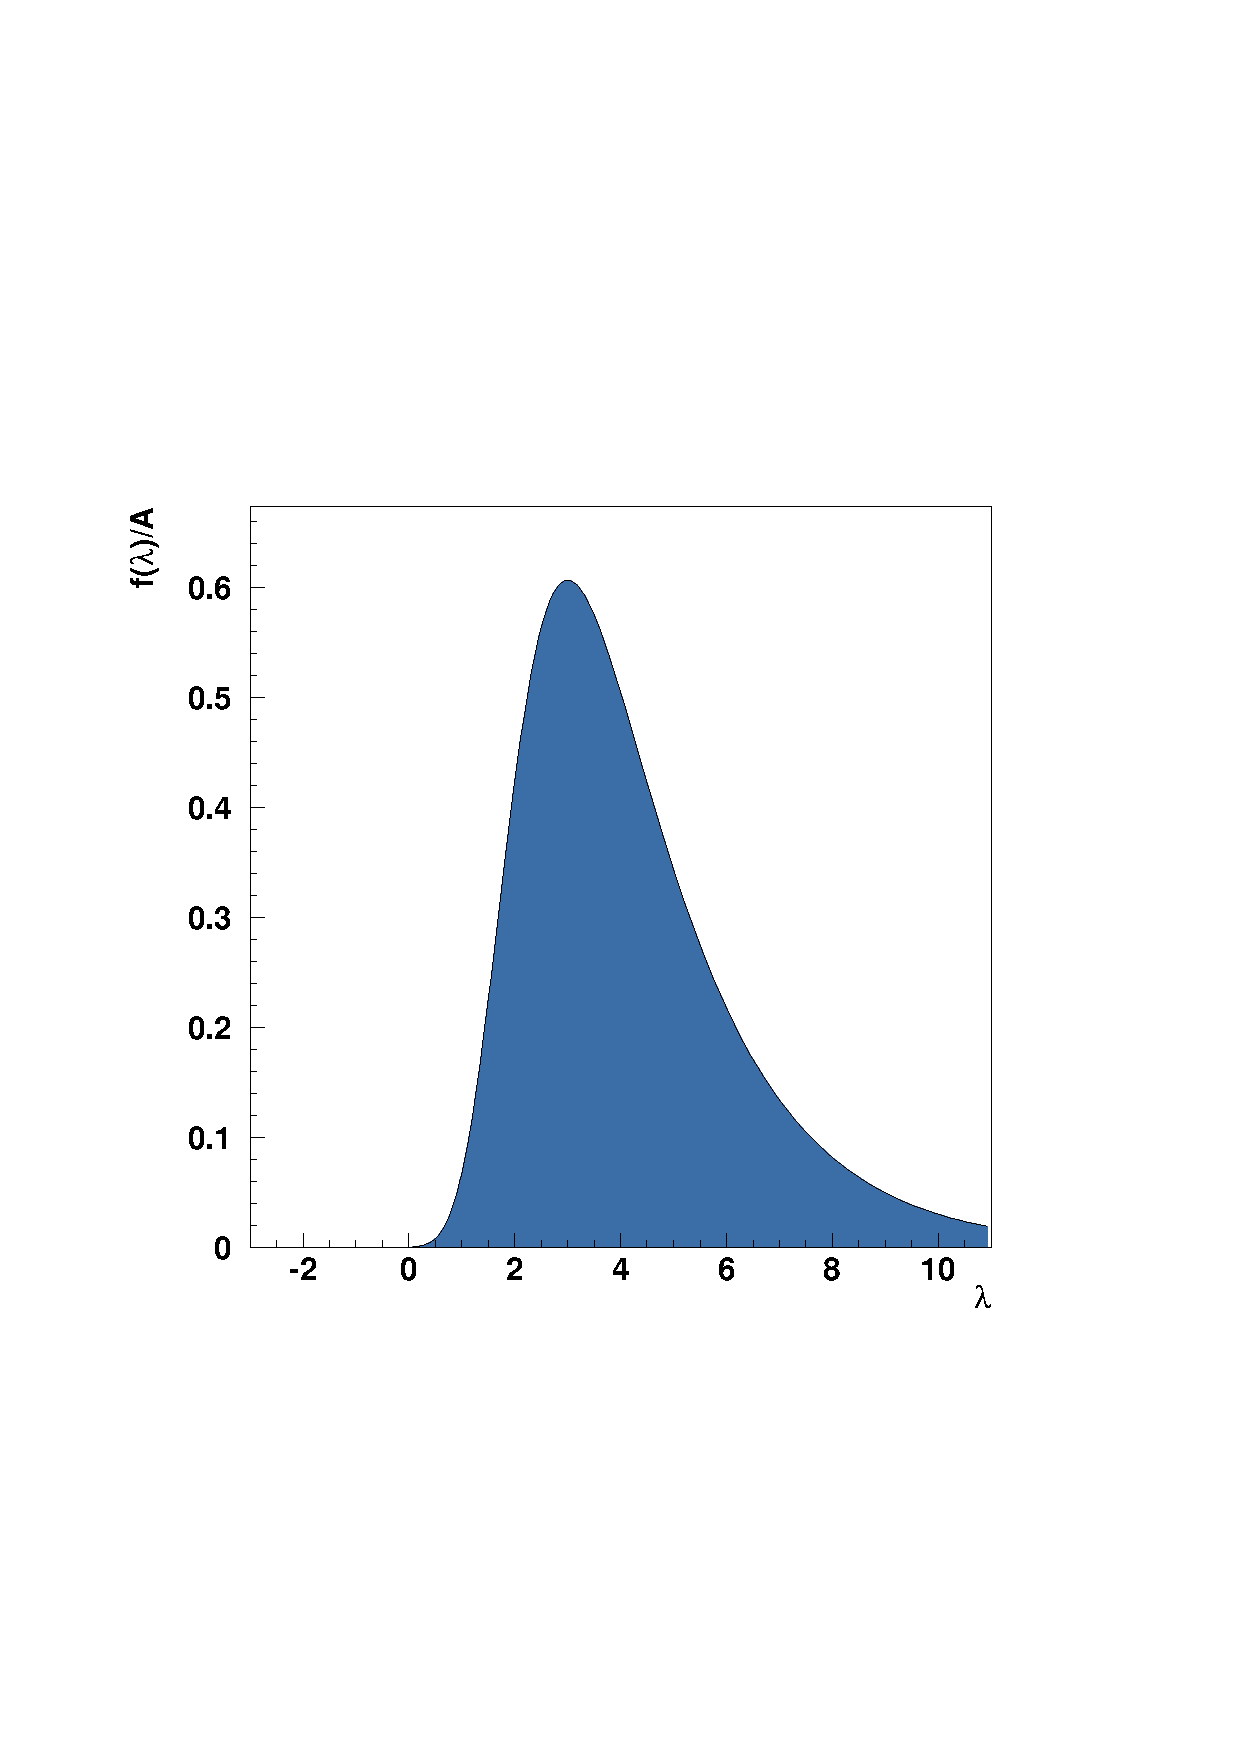
\includegraphics[width=0.55\textwidth]{cap4/immagini/landau.pdf}
%  \caption{\it Simplified Landau function~\ref{eq:landau} plotted against $\lambda$.}\label{fig:landau}
%\end{figure}
%to be compared with the result of the experimental distribution after the
%pedestal subtraction \fig{fig:ph}. 
%\begin{figure}[!htbp]
%  \includegraphics[width=0.4\textwidth]{cap4/immagini/ph.pdf}
%  \caption{\it Example of pulse height distribution. }\label{fig:ph}
%\end{figure}
%
%The stochastic nature of the channel noise affects the experimental pull
%distribution overlapping the expected Landau with a gaussian centered around
%zero. This results in the typical pattern for a depleted silicon and low LET
%particles shown in~\fig{fig:pull}.\\
%%The experimental pull distribution for a depleted silicon and low LET particles
%%shows a typical pattern~\fig{fig:ph}. This is the result of the overlapping of
%%two distributions:
%%The stochastic nature of the channel noise affects
%%In the case of a depleted silicon and low LET particles, the pull
%%distribution~\fig{fig:ph} shows a typical pattern, with two peaks.
%%Despite the pedestal subtraction
%%This is the result of the overlapping of two different distribution
%%The high
%%energy peak is the expected most probable value of the Landau distribution while
%%the low energy one is due to the channel noise, that follows a gaussian
%%distribution around zero.\\
%A threshold in the trigger is set in order to exclude the noise events. In order
%to do that we inspect the {\it pull} distribution for each channel~\fig{fig:pull}. The pull is defined as the
%ratio between the pulse heigh of the strip with the maximum signal in the event
%and its corresponding noise.
%\begin{equation}
%{\rm PULL} = \frac{{\rm ADC}_{i(max)}}{{\rm RMS}_{i(max)}}
%\end{equation}
%\begin{figure}[!htbp]
%  \includegraphics[width=0.4\textwidth]{cap4/immagini/pull.pdf}
%  \caption{\it Example of pull distribution. }\label{fig:pull}
%\end{figure}
%%
%%(MIPs?)
%


\subsection{Gain equalisation}
A channel to channel correction has to be applied since one expects gain
variations of the order of 15\% {\color{red}  qui immagine che mostra questo valore} across the channels of each chip. The relative
gain of each channel is determined finding the most probable deposited energy
value $E_{\rm mp}$ with a Landau fit of the energy spectrum for
each channel.\\
The procedure for the gain equalisation is the following:
\begin{itemize}
\item the most probable value of the pulse height distribution for each strip is
  computed using the simplified Landau distribution~\eq{eq:landau};
\item one of the strips is taken as a reference and the values of all the
  remaining strips are rescaled to the reference.
\end{itemize}
After this equalisation the most probable value of the ADC distribution is
stable within a few percent.
%\begin{figure}[!htbp]
%  \centering 
%  \includegraphics[width=0.5\textwidth]{cap4/equal_landau.jpg}
%  \caption{\textit{dopo equalizzazione}.}
%  \label{fig:equalised}
%\end{figure}


\subsection{Cluster detection}\label{subs:cluster}
A cluster is defined as a group of contiguous channels detecting the passage of
the same particle. The channel with the largest signal is referred to as the
{\it seed}. To define a cluster in the analysis a cut is applied: channels whose
pull exceeds the threshold are considered ``active''~(\fig{fig:cluster_a}). Two
active channels that are separated by one or more ``inactive'' channels are
part of different clusters~(\fig{fig:cluster_b}).
\begin{figure}[!htbp]
  \centering 
  \subfloat[] {\includegraphics[width=.45\textwidth]{cap4/immagini/1cluster_profile-crop.pdf}\label{fig:cluster_a}}\quad
  \subfloat[] {\includegraphics[width=.45\textwidth]{cap4/immagini/2cluster_profile-crop.pdf}\label{fig:cluster_b}}
  \caption{\textit{Example of a one-cluster (a) and two-cluster (b) event. In
      blue the signal value for each channel, in red the selection cut (in this
      case 10 $RMS_{\rm channel}$).}}
  \label{fig:cluster}
\end{figure}
Since each cluster corresponds to a different particle hit, the exact hit position
can be determined by the average of the positions of the cluster strips weighted by the corresponding PH value:
\begin{equation}\label{eq:cog}
x_{cm} = \frac{\sum_{i\in{\rm cluster}} x_i\cdot {\rm PH}_i}{\sum_{i\in{\rm cluster}} {\rm PH}_i}
\end{equation}
Effects that contribute to the cluster size are due to charge sharing and
electronics crosstalk. The former depends on processes where the charge is
shared among contiguous channels while the latter is independent on the position
where the charge was generated. The angle of the incoming particle in the
coordinate system of the crossed detector is thus relevant for the cluster shape
and
the deposited charge.\\

Some relevant features of the cluster in silicon microstrip detectors are the following:
\begin{itemize}
\item {\bf Cluster size}. From geometrical considerations it is possible to
  connect the angle $\theta$ at which the particle hits the detector with the
  number $N_{\rm strip}$ of strips that collect its deposited charge~\cite{Turchetta:1993vu}:
\begin{equation}
N_{\rm strip} = \frac{d}{p}\tan{\theta}
\end{equation}
where $d$ is the detector thickness and $p$ the strip pitch. As a result, for
particles that hit the detector perpendicularly or with a small angle the
charge is usually collected by one or two strips: this can be observed in~\fig{fig:nrstrip}.
Nevertheless particles with a larger angle and the presence of capacitive effects can generate larger clusters.
\item {\bf Amplitude}. A particle crossing two or more channels releases its
  energy among the strips. The total deposited energy is then proportional to the sum
  of the signal read by the cluster channels~(\fig{fig:amplitude})
\begin{equation}
Amplitude_{\rm cluster} = \sum_{i\in {\rm cluster}} PH_i
\end{equation}\label{eq:cluster_amplitude}
which is expected to be distributed according to a Landau distribution.
\begin{figure}[!htbp]
  \centering 
  \subfloat[] { \includegraphics[width=0.5\textwidth]{cap4/immagini/nrstrip_cluster-crop.pdf}\label{fig:nrstrip} }
  \subfloat[] { \includegraphics[width=0.5\textwidth]{cap4/immagini/amplitude_cluster-crop.pdf}\label{fig:amplitude} }\\
  \subfloat[] {\includegraphics[width=0.5\textwidth]{cap4/immagini/snr_cluster-crop.pdf} \label{fig:snr} }
  \subfloat[] { \includegraphics[width=0.5\textwidth]{cap4/interstrip.jpg}  \label{fig:interstrip} }
  \caption { {\it Distribution of the cluster size (a), total cluster
      amplitude (b), signal to noise ratio (c) and interstrip distribution of
      the center of gravity (d).} }
\end{figure}

\item {\bf SNR}. The signal to noise ratio (SNR) is a key parameter for the
  tracking performance. A large SNR ensures a high efficiency for the hit
  reconstruction and allows the measurement of charge sharing between
  neighbouring strips, improving the resolution through the calculation of the
  charge barycenter~(\eq{eq:cog}). The cluster SNR (\fig{fig:snr}) is computed as the sum
  of the cluster signals divided by the square sum of the RMS noise value of all
  the strips in the
  cluster itself:
\begin{eqnarray}
SNR &=& \frac{Amplitude_{\rm cluster}}{noise_{\rm cluster}} \label{eq:cluster_snr}\\
noise_{\rm cluster} & = & \sqrt{\frac{\sum_{i\in {\rm cluster}} RMS_i^2}{N}}\label{eq:cluster_noise}
\end{eqnarray}
where $N$ is the number of strips composing the cluster and $RMS_i$ is the strip
noise defined in~\eq{eq:rms_cm_sub}.

\begin{figure}
  \centering 
  \subfloat[] { \includegraphics[width=.7\textwidth]{tikz/uniform_diffusion.tikz} \label{fig:uniform_diffusion}}\\
  \subfloat[] {  \includegraphics[width=.7\textwidth]{tikz/gaussian_diffusion.tikz} \label{fig:gaussian_diffusion}}
  \caption{ \it In the case of a uniform charge distribution (a) a particle
    crossing the detector at $3/4$ of the distance between two strips release
    $1/4$ ot the charge on the left strip and $3/4$ on the right one. In the
    case of a gaussian charge distribution (b) the left strip collect only $1/5$
    of the signal and the right one $4/5$. The dotted line represents the
    separation between the two strips.}

\end{figure}

\item {\bf Spatial distribution}. Because of charge sharing effects, the
  determination of the cluster center of gravity according to~\eq{eq:cog} is
  biased. Observing the plot of the interstrip hit
  position~(\fig{fig:interstrip}) in fact, the distribution is not flat: this is
  due to the non-linearity of the
  charge division between channels.\\
  To better understand this effect consider the different effect one can
  consider the cases of a uniform~(\fig{fig:uniform_diffusion}) and
  gaussian~(\fig{fig:gaussian_diffusion}) charge distribution and a particle
  crossing the detector at $3/4$ of the distance between two
  strips. In the uniform distribution case the left and right strips collect
  $1/4$ and $3/4$ of the total deposited charge,
  so that the center of gravity algorithm returns the correct position. In the case
  of a gaussian charge distribution, nevertheless, the left strip collects roughly
  $1/5$ of the total charge and the right $4/5$: the larger weight of the right strip
  moves $x_{cm}$ towards right.\\
  In section~\ref{sect:eta_correction} an algorithm that allows to correct for
  this bias is discussed.
\end{itemize}



{\color{red} mettere plot che mostrno come abbassando il taglio i cluster hanno piu' strip}
An explorative study on the dependance of cluster features on the selection cut
has been performed. As expected the higher the cut the smaller the cluster size
and the amplitude. %The best SNR is reached with a cut around {\bf qui quanto}
%while the $\eta$ distribution {\bf qui qualche considerazione}.
\begin{figure}[!htbp]
  \centering 
  \subfloat[] { \includegraphics[width=0.35\textwidth]{fig:snr_cut0.jpg} }
  \subfloat[] { \includegraphics[width=0.35\textwidth]{fig:snr_cut1.jpg} }\\
  \subfloat[] { \includegraphics[width=0.35\textwidth]{fig:snr_cut2.jpg} }
  \subfloat[] { \includegraphics[width=0.35\textwidth]{fig:snr_cut3.jpg} }
  \caption{ {\it Cluster SNR.}}
  \label{fig:clusteramplitude}
\end{figure}


\subsection{$\eta$ distribution}\label{sect:eta}
Due to capacitive coupling among the strips the charge deposited by the passage
of a particle is shared between neighbouring channels. It is important to
estimate this effect, since it affects the detector behaviour. A
description of the non-linearity of the charge division is given by the $\eta$
distribution. For each event the quantity $\eta$ is defined as
\begin{equation}
\begin{displaystyle}
  \eta = \left\{
  \begin{array}{ll}
    \frac{{\rm PH}_i-{\rm PH}_{i+1}}{{\rm PH}_i+{\rm PH}_{i+1}} & {\rm if}\quad PH_{i+1} > PH_{i-1}\\[8pt]
    \frac{{\rm PH}_{i-1}-{\rm PH}_{i}}{{\rm PH}_{i-1}+{\rm PH}_{i}} & {\rm otherwise}
  \end{array}
\right.
\end{displaystyle}
\end{equation}
where $i$ is the strip in the cluster with the largest value. The $\eta$ quantity can
be interpreted as follows:
\begin{itemize}
\item if one channel collects almost the whole
signal then $\eta \sim -1$ or $\eta \sim 1$;
\item if the charge is equally shared on two channels then $\eta \sim 0$.
\end{itemize}
From a practical point of view, one computes $\eta$ only inside a cluster. This
ensure that al least one among ${\rm PH}_{i-1}$ and ${\rm PH}_{i+1}$ exists,
nevertheless it implies that $\eta = \pm 1$ almost never happens. As an
alternative it is also possible to consider events where a single strip
overcomes the threshold set to identify the hit strips, and set a lower
threshold on the neighbours. \fig{fig:eta_ok} shows the typical plot of the
$\eta$ function.\\
The most probable value and the width of the two peaks of the $\eta$
distribution depend on the physical features of the detector, such as the
thickness, the strip pitch and the applied voltage. In~\fig{fig:eta_angolo} the
same detector of~\fig{fig:eta_ok} has been used, but its axis is no longer
parallel to the beam axis.\\
\begin{figure}[!htbp]
  \centering 
  \subfloat[] {\includegraphics[width=0.49\textwidth]{cap4/immagini/eta_separata-crop.pdf}\label{fig:eta_ok}}
  \subfloat[] {\includegraphics[width=0.49\textwidth]{cap4/immagini/eta_vicina-crop.pdf}\label{fig:eta_angolo}}
  \caption{\textit{Examples of eta distribution. In figure (a) two peaks around $\pm$1 are evindent: almost all the charge has been collected in one channel. Figure (b) shows a case where there is no net collection of charge on one channel}.}
\label{fig:eta}
\end{figure}
In the floating strip readout mode if a particle hits a floating strip a
fraction almost equal of the signal is collected by the two nearby readout
ones. In this case one would then expect a large fraction of events with
$\eta\neq\pm 1$. This is indeed the case, as shown in~\fig{fig:eta_floating}: 
one further peak per non-readout
strip appears in the $\eta$ distribution.\\
\begin{figure}[!htbp]
  \centering 
  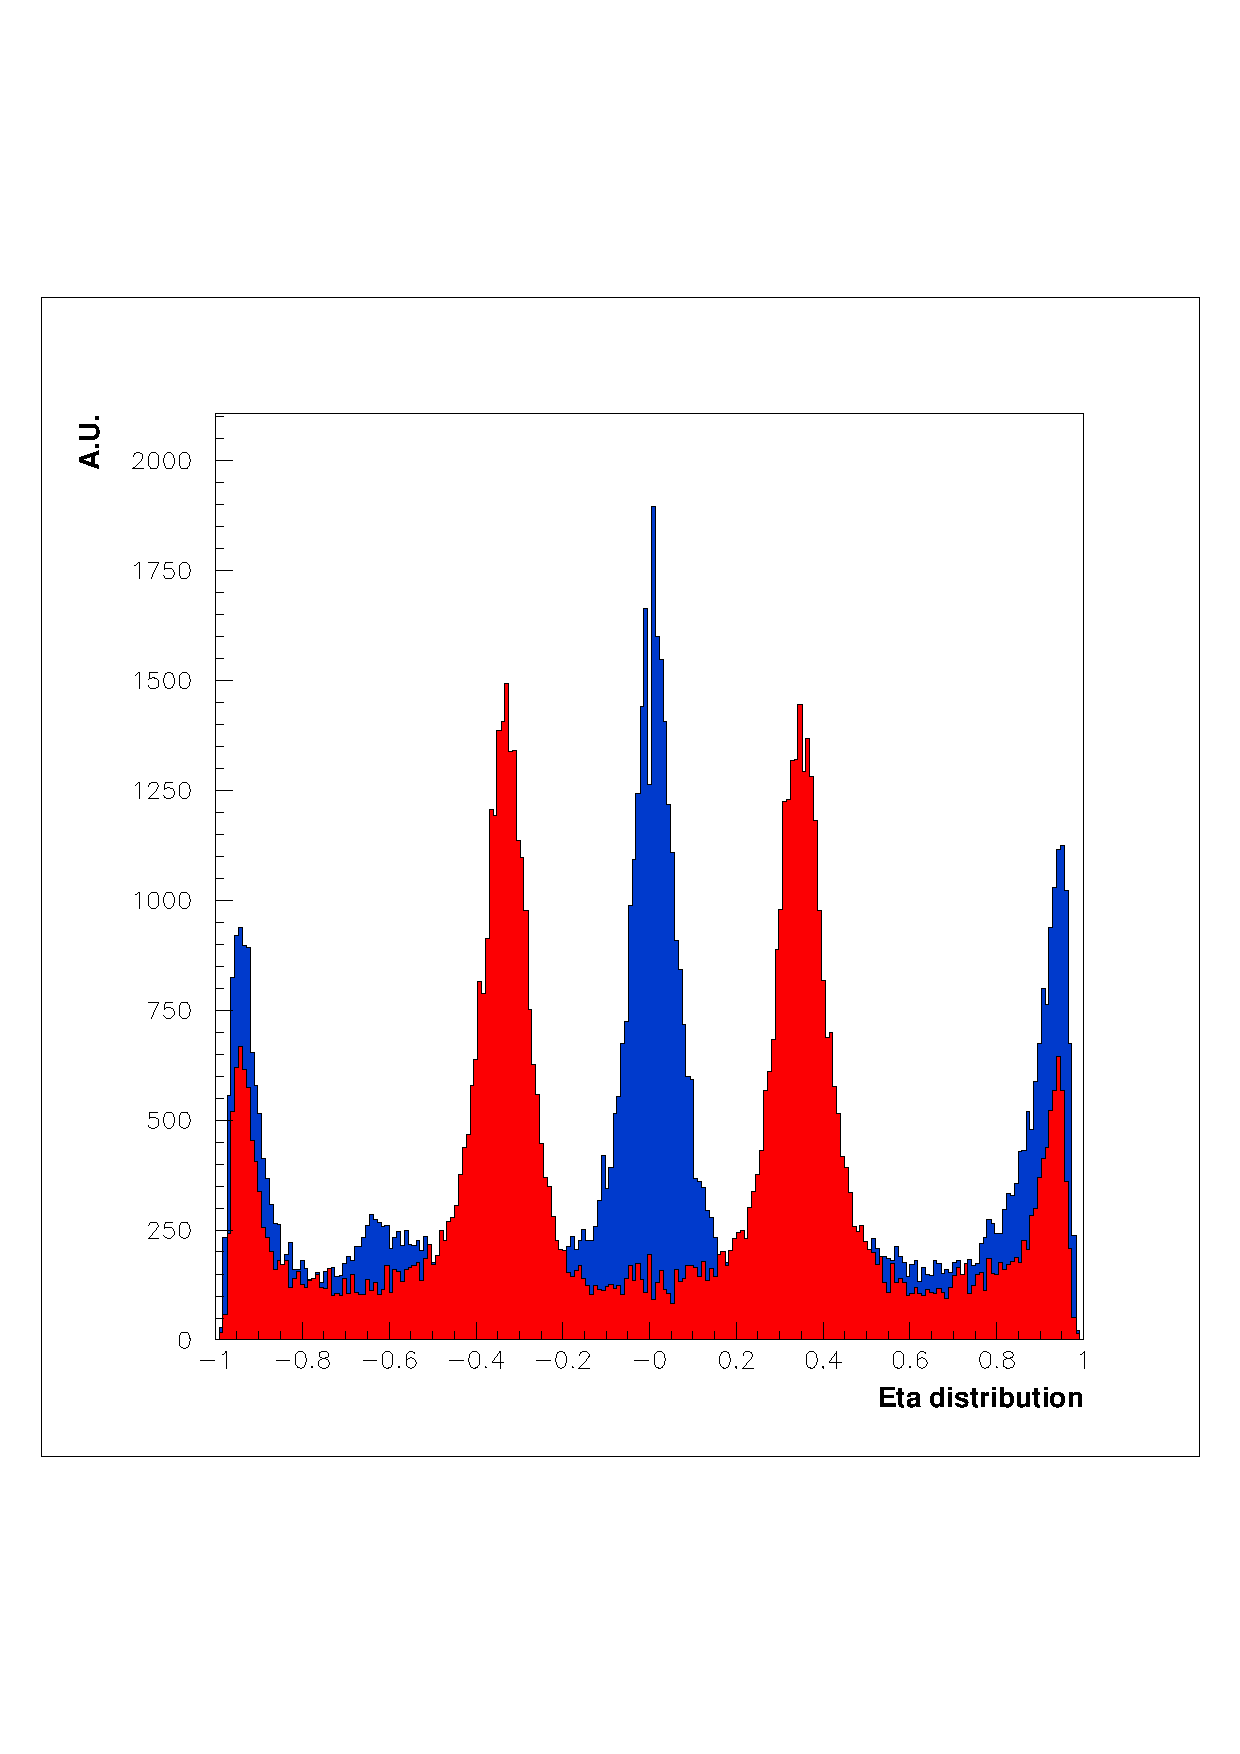
\includegraphics[width=0.49\textwidth]{cap4/immagini/eta_floating.pdf}
  \caption{\textit{The $\eta$ distribution presents as many further
      peaks as many floating strips are present. Red: one readout
      strip and one floating. Blue: one readout strip and two
      floating.}}
  \label{fig:eta_floating}
\end{figure}
Since the $\eta$-value is related to the main geometrical and electrical
parameters of the detectors, it is a good probe to check the correct detector
response: an asymmetric $\eta$ indicates an incorrect sampling of the analog
signal since the deposited charge is thus not equally shared among the
strips. This effect can be further studied inspecting the lateral pull
distribution (\fig{fig:pull_laterale}), i.e. the pull distributions of the
strips adjacent to the one with the maximum signal.
\begin{figure}[!htbp]
  \centering 
  \subfloat[]{ \includegraphics[width=0.49\textwidth]{cap4/immagini/pull_laterale_ok.pdf}\label{fig:pull_laterale_ok} }
  \subfloat[]{ \includegraphics[width=0.49\textwidth]{cap4/immagini/pull_laterale_nok.pdf}\label{fig:pull_laterale_nok} }
  \caption{\textit{\color{red}A comparison of the lateral pull distribution (x and y) }}
  \label{fig:pull_laterale}
\end{figure}
If the signal is sampled correctly the left and right pull distributions are
similar (\fig{fig:pull_laterale_ok}), giving rise to a symmetric $\eta$
distribution. If the signal is not sampled correctly the distributions differ (\fig{fig:pull_laterale_nok})
showing that the deposited charge is not equally shared among the
strips. {\color{red}Dire che e' legato al clock di sampling?}




\section{Microstrip silicon detectors for multi-tracking}
The main goal of this part of my research activity is the study of microstrip
silicon detectors as high spatial resolution detectors to reconstruct tracks in
multi-particle events. Nowadays microstrip silicon detectors are the most common
devices to reconstruct particle trajectories, because of many reasons:
\begin{itemize}
\item ability to reconstruct the spatial position with a few micron accuracy;
\item small thickness which allows to absorb just a small fraction of the particle energy thus
  introducing minimum perturbation of the particle trajectory;
\item temporal resolution of a few nanoseconds.
\end{itemize}
The spatial resolution is clearly the most important parameter for tracking.  A
practical definition the of impact parameter resolution for a multiple module
detector is based on the reconstruction of single cluster tracks
(\fig{tikz:track_reconstruction}). In absence of any magnetic field the
particles travel in a straight line, thus the reconstruction can be performed
via a linear fit ot the impact positions. Defining the {\em residuals} as the
difference between the impact point and its reconstructed position, the
residuals distribution describes how precisely the trajectory is reconstructed;
its standard deviation can be interpreted
as the impact parameter resolution of the detector~\cite{Turchetta:1993vu}.\\
\begin{figure}[!htbp]
\centering
\begin{tikzpicture}[scale=.5,every node/.style={minimum size=1cm},on grid,every text node part/.style={align=center}]
  
% % track
\begin{scope}
 \draw[dashdotted] (-2,1) -- (18,5) node[right] {particle\\track};
\end{scope}

 % projection
\begin{scope}[ yshift=-20, xslant=2]
  \draw[,domain=-2:14,variable=\x,red] plot ({\x},{0.5+2.0/15.0*\x})  node[right,black] {track\\projection};
\end{scope}

% modules
\begin{scope}[ yslant=0., yslant=0.5]
 \draw[draw=none,fill=white] (0,0) rectangle ({2*.5+.25},5);
\draw (0,0) -- (0,5) -- (5,5) -- (5,0) -- (0,0);
\foreach \i in {0,1,...,9}
\draw ({.5*\i},0) -- ( {.5*\i},5) ;
\end{scope}

\begin{scope}[ xshift = 170, yslant=0.5]
 \draw[draw=none,fill=white] (0,0) rectangle ({5*.5+.25},5);
  \draw (0,0) -- (0,5) -- (5,5) -- (5,0) -- (0,0);
  \foreach \i in {0,1,...,9}
  \draw ({.5*\i},0) -- ( {.5*\i},5) ;
\end{scope}

\begin{scope}[ xshift = 340, yslant=0.5]
  \draw[draw=none,fill=white] (0,0) rectangle ({8*.5+.25},5);
  \draw (0,0) -- (0,5) -- (5,5) -- (5,0) -- (0,0);
  \foreach \i in {0,1,...,9}
  \draw ({.5*\i},0) -- ( {.5*\i},5) ;
\end{scope}


\begin{scope}[ yshift=-20, xslant=2]
    \fill [blue] (0,{2*.25}) rectangle (.5,{(2+1)*.25}) node [below right, black] {$x_1$};
    \draw (0,0) -- (.5,0) -- (.5,2.5) -- (0,2.5) -- (0,0);
    \foreach \i in {1,...,9}
    \draw (0,{.25*\i},0) -- (0.5,{.25*\i}) ;
  \end{scope}

 \begin{scope}[ xshift = 170, yshift=-20, xslant=2]
    \fill [blue] (0,{5*.25}) rectangle (.5,{(5+1)*.25}) node [below right, black] {$x_2$};
   \draw (0,0) -- (.5,0) -- (.5,2.5) -- (0,2.5) -- (0,0);
   \foreach \i in {1,...,9}
   \draw (0,{.25*\i},0) -- (0.5,{.25*\i}) ;
 \end{scope}

 \begin{scope}[ xshift = 340, yshift=-20, xslant=2]
    \fill [blue] (0,{8*.25}) rectangle (.5,{(8+1)*.25}) node [below right, black] {$x_3$};
   \draw (0,0) -- (.5,0) -- (.5,2.5) -- (0,2.5) -- (0,0);
   \foreach \i in {1,...,9}
   \draw (0,{.25*\i},0) -- (0.5,{.25*\i}) ;
 \end{scope}


\end{tikzpicture}

\caption{{\it A particle crossing the detector and its projection}}\label{tikz:track_reconstruction}
\end{figure}
The impact parameter resolution depends not only on the intrinsic sensor
resolution but also on the precise alignment of the whole detector and on the
multiple scattering of the materials. These
parameters can be optimised independently in order to achieve the best
resolution. The optimisation follows a two steps procedure:
\begin{itemize}
\item optimisation of the planes alignment;
\item optimisation of the impact point detection.
\end{itemize}


%In the first part of the analysis only the events with a single clusters were
%used, since they can be associated associated with the track produced by a
%unique particle. Once we have fully carachterised the detectors we will explore
%multi-particle track reconstruction.

\subsection{The alignment procedure}
Even though built with high precision, in a detector system with multiple
modules some misalignment between the modules can happen
(\fig{fig:module_misalignment}). In order not to introduce a systematic bias
while evaluating the system resolution it is necessary to align all the modules
to a reference frame (\fig{fig:module_alignment}) introducing an offset in the coordinate system for each module.\\
\begin{figure}[!htbp]
  \centering 
  \subfloat[] { \begin{tikzpicture}[scale=.4,every node/.style={minimum size=1cm},on grid,every
  text node part/.style={align=center}, declare function={ track(\x) = 1.+3.0/7.5*\x; }]

  % original, misaligned
  \def \a {0}
  \def \b {.8}
  \def \c {-.8}

  \begin{scope}
    % axis
    \draw[->] (-1,-1) -- (11,-1) node[right] {z};
    \draw[->] (0,-2) -- (0,7) node[above] {x};

    % track
    \draw[,domain=-.5:10,variable=\x,red] plot ({\x}, {track(\x)} );

    % m1
    \draw[dashed] (2.25,-1) -- (2.25,1) node[below=1] {$z_1$};
    \fill[blue] (2,{track(2)+\a}) rectangle (2.5,{track(2.5) +\a});
    \draw[dotted] (0,1) -- (2,1);
    \draw[thick] (2,{1 +\a}) rectangle (2.5,{5 +\a})  node[above] {$M_1$};
    
    % m2
    \draw[dashed] (5.25,-1) -- (5.25,{1+\b}) node[below=1.3] {$z_2$};
    \fill[blue]  (5,{track(5) +\b}) rectangle (5.5,{track(5.5) +\b});
    \draw[dotted] (0,{1+\b}) -- (5,{1+\b});
    \draw[thick] (5,{1 +\b})          rectangle (5.5,{5 +\b})  node[above] {$M_2$};
    
    % m3
    \draw[dashed] (8.25,-1) -- (8.25,{1+\c}) node[below=.75] {$z_3$};
    \fill[blue]  (8,{track(8) +\c}) rectangle (8.5,{track(8.5) +\c});
    \draw[dotted] (0,{1+\c}) -- (8,{1+\c});
    \draw[thick] (8,{1 +\c})          rectangle (8.5,{5 +\c})  node[above] {$M_3$};
  \end{scope}
  
\end{tikzpicture}
 \label{fig:module_misalignment}}
  \subfloat[] { \input{tikz/module_alignment_b.tikz} \label{fig:module_alignment}}
  \caption{ \it Small misalignments between detector modules that affect the
    track reconstruction cannot be avoided (a) when building the detector. A
    software procedure can effectively improve the alignment. In all the
    following figures $z$ represents the position along the beam axis.
%  \caption{\it {In the ideal case (a) the modules are perfectly aligned: in blue
%      the expected hit points. In the real world nevertheless the exact
%      alignment isn't achievable (b): the particle traverse the detector in slightly
%      different positions.}
  }\label{tikz:module_alignment}
\end{figure}
The zero step required to align the system is to select one of the modules as
the absolute reference frame: all the remaining modules will be aligned with
respect to it. In the following module $M_1$ (\fig{tikz:module_alignment}) will
be taken as the reference. The alignment procedure has been performed with the
detector perpendicularly aligned with respect to the beam axis in such a way
that the distribution of angular coefficients of the tracks is symmetric around
zero.\\
\begin{figure}[!htbp]
  \centering 
  \subfloat[] { \input{tikz/align13a.tikz} \label{fig:align13_a}}
  \subfloat[] { \begin{tikzpicture}[scale=.4,every node/.style={minimum size=1cm},on grid,every
  text node part/.style={align=center}, declare function={ track(\x) =
    1.+3.0/7.5*\x; trackb(\x) = 1.9+.4/1.5*(\x-2.25); }]
  
  \def \a {.0}
  \def \c {-.8}

  % aligned
  \begin{scope}
    % axis
     \draw[->] (-1,-1) -- (11,-1) node[right] {z};
    \draw[->] (0,-2) -- (0,7) node[above] {x};

    % angle & track
    \shade[left color=white,right color=red!50!white ] (3.5,{track(3.5)}) --
    ({3.5+2},{track(3.5)}) arc (0:21.8:2)  -- cycle;
    \draw[red] (3.5,{track(3.5)}) -- (6.5,{track(3.5)})  node[below left] {$\alpha'$};
    \draw[red,domain=-.5:10,variable=\x] plot ({\x}, {track(\x)} );

    % m1
    \draw[dashed] (2.25,-1) -- (2.25,1) node[below=1] {$z_1$};
    \draw[dashed] (2.25,{track(2.25)} ) --  (0,{track(2.25)}) node[left] {$x_1$};
    \fill[blue] (2,{track(2)}) rectangle (2.5,{track(2.5)});
    \draw[thick] (2,1) rectangle (2.5,5)  node[above] {$M_1$};
        
    % m3
    \draw[dashed] (8,{track(8.25)} ) -- (0,{track(8.25)}) node[left] {$x_3'$};    
    \draw[dashed] (8.25,-1) -- (8.25,1) node[below=1] {$z_3$};

    \fill[red!30!white]  (8,{track(8) +\c}) rectangle (8.5,{track(8.5) +\c});
    \draw[thick,dotted,red] (8,{1 +\c})          rectangle (8.5,{5 +\c});

    \fill[blue]  (8,{track(8)}) rectangle (8.5,{track(8.5)});
    \draw[thick] (8,1)          rectangle (8.5,5)  node[above] {$M_3$};
  \end{scope}
  
\end{tikzpicture}
 \label{fig:align13_b}} 
  \caption{\it If the modules are aligned the angular distribution of the tracks
    $\tan{\alpha}$ has to be symmetrical around 0, but this (a) is usually not
    the case. The introduction of the software alignment (\eq{eq:correzione3})
    allows to restore the correct alignement (b).}
  \label{fig:align13}
\end{figure} 
Using modules $M_1$ and $M_3$ (\fig{fig:align13}), the
angular coefficient for each (1-cluster) track is computed:
\begin{equation}\label{eq:m13}
m_{1,3} = \frac{x_3-x_1}{z_3-z_1} = \tan{(\alpha)}
\end{equation}
$x_1$ and $x_3$ being the impact point on $M_1$ and $M_3$ respectively, and $z_1$
and $z_3$ the position along the beam axis.  If the detectors are not perfectly
aligned the initial distribution is not centered around zero
(\fig{fig:align13_a}). This effect can be corrected (\fig{fig:align13_b})
introducing an offset $\Delta_3$ so that
\begin{eqnarray}
x_3' & = & x_3 + \Delta_3 \label{eq:correzione3}\\
m'_{1,3} &=& \frac{x'_3-x_1}{z_3-z_1} = \tan{(\alpha')}\label{eq:m13corretta}
\end{eqnarray}
\begin{figure}[!htbp]
  \centering 
  \subfloat[] { \includegraphics[width=0.5\textwidth]{cap4/immagini/before_align3.jpg} }
  \subfloat[] { \includegraphics[width=0.5\textwidth]{cap4/immagini/after_align3.jpg} }\\
  \caption{ {\it Angular distribution of the tracks before (a) and after (b) the
    alignment procedure.}}
  \label{fig:tan_alpha}
\end{figure}
The angular coefficient distribution is recomputed using \eq{eq:m13corretta}:
\fig{fig:tan_alpha} shows the result.\\
\begin{figure}[!htbp]
  \centering 
  \subfloat[] { \input{tikz/align2a.tikz} \label{fig:align2_a} }
  \subfloat[] { \begin{tikzpicture}[scale=.4,every node/.style={minimum size=1cm},on grid,every
  text node part/.style={align=center}, declare function={ track(\x) =
    1.+3.0/7.5*\x; trackb(\x) = 1.9+.4/1.5*(\x-2.25); }]
  
  \def \a {.0}
  \def \b {.8}

  % aligned
  \begin{scope} [xshift = 520]

   % axis
    \draw[->] (-1,-1) -- (11,-1) node[right] {z};
    \draw[->] (0,-2) -- (0,7) node[above] {x};

    % track
    \draw[red,domain=-.5:10,variable=\x] plot ({\x}, {track(\x)} ) ;

    % m1
%    \draw[dashed] (2.25,{track(2.25)} ) --  (0,{track(2.25)}) node[left] {$x_1$};
    \draw[dashed] (2.25,-1) -- (2.25,1) node[below=1] {$z_1$};
    \fill[blue] (2,{track(2)}) rectangle (2.5,{track(2.5)});
    \draw[thick] (2,1) rectangle (2.5,5)  node[above] {$M_1$};
    

    % m2

    \fill[red!50!white] (5,{track(5)+\b}) rectangle (5.5,{track(5.5)+\b});
    \draw[thick,red,dotted] (5,{1+\b}) rectangle (5.5,{5+\b});


    \draw[dashed] (5.25,{track(5.25)} ) --  (0,{track(5.25)}) node[left] {$x_2'=x_2+\Delta_2$};
    \draw[dashed] (5.25,-1) -- (5.25,{1}) node[below=1] {$z_2$};
    \fill[blue] (5,{track(5)}) rectangle (5.5,{track(5.5)});
    \draw[thick] (5,1) rectangle (5.5,5)  node[above] {$M_2$};

    % m3
%    \draw[dashed] (8,{track(8.25)} ) -- (0,{track(8.25)}) node[left] {$x_3$};    
    \draw[dashed] (8.25,-1) -- (8.25,1) node[below=1] {$z_3$};
    \fill[blue]  (8,{track(8)}) rectangle (8.5,{track(8.5)});
    \draw[thick] (8,1)          rectangle (8.5,5)  node[above] {$M_3$};
  \end{scope}
  
\end{tikzpicture}
 \label{fig:align2_b} }
  \caption{\it Due to the detector misalignment the impact point $x_2$ and the
    reconstructed position $x_2^*$ differs (a). An offset $\Delta_2$ has to be
    introduced to remove the systematic error (b).}
  \label{fig:align2}
\end{figure} 
Using $m'_{1,3}$ it is
possible to estimate the theoretical impact point $x_2^*$ on $M_2$ (\fig{fig:align2_a}):
\begin{equation}\label{eq:x2_teorico}
x_2^* = m'_{1,3}\cdot z_2 + x_1
\end{equation}
Such a value can be used to estimate the misalignment of $M_2$ computing the
distribution of the {\em residuals} i.e. the difference between the estimated
point $x_2^*$ and the actual impact point $x_2$:
\begin{equation}
{\rm res}_2 = x_2-x_2^*
\end{equation}

\begin{figure}[!htbp]
  \centering 
  \subfloat[] { \includegraphics[width=0.5\textwidth]{cap4/immagini/before_align2.jpg} }
  \subfloat[] { \includegraphics[width=0.5\textwidth]{cap4/immagini/after_align2.jpg} }\\
  \caption{ {\it Distribution of the residuals before (a) and after (b) the
      software alignment procedure.}}
  \label{fig:tan_alpha}
\end{figure}

\fig{fig:residui} shows an example of such a distribution. The mean value of the
residual distribution $\Delta_2$ can be used as an offset to correct for the
misalignment (\fig{fig:align2_b}):
\begin{equation}
x_2'  =  x_2 + \Delta_2
\end{equation}
The new determined impact points ($x_1$,$z_1$),($x_2'$,$z_2$),($x_3'$,$z_3$) can be
finally used to reconstruct the particle trajectory via a linear fit.


\subsection{The $\eta$ correction}\label{sect:eta_correction}
As shown in section~\ref{subs:cluster} the use of the center of gravity
method~\eq{eq:cog} to estimate the particle impact point is biased due to
charge sharing effect. Considering a two-strip cluster, for example, it is
possible to write the reconstructed hit point $x_{cm}$ in terms of the $\eta$ quantity:
\begin{equation}\label{eq:cm_eta}
x_{cm} = x_L+p \left(1+\eta\right)
\end{equation}
where $x_L$ is the position of the left strip and $p$ the strip pitch.\\
It is trivial to verify that if $\eta=-1(1)$ the left (right) strip collected
the whole charge and $x_{cm} = x_{L(R)}$ while if $\eta=0$ the charge is equally
shared, corresponding to a particle in the middle ($x_{cm} =
x_{L}+p/2$). \fig{fig:interstrip_biased} shows in fact that the interstrip
distribution agrees with the $\eta$ distribution (\fig{}).\\
The nonlinearity in the charge sharing results in a systematic shift in the
reconstructed hit position that in turn worsen the estimation of the detector
spatial resolution.\\
In order to correct the reconstructed position a dedicated procedure is
required. A more general form of~\eq{cm-eta} is
\begin{equation}\label{eq:eta_correction}
x_{\rm pos} = x_L+f(\eta) \cdot p
\end{equation}
with $f(\eta)$ satisfying the following conditions:
\begin{itemize}
\item if the whole charge is collected on the left strip $\eta=-1$ and $x_{\rm
    pos} = x_L$ requires that $f(-1)=0$;
\item if the whole charge is collected on the right strip $\eta=1$, and $x_{\rm
    pos} = x_L+p = x_R$ requires that $f(1)=1$;
\item if the same fraction of the charge is collected on the two strips $\eta=0$
  and $x_{\rm pos} = x_L+p/2 = (x_L + x_R)/2$ requires that $f(0) = 1/2$.
\end{itemize}
Due to the non-linearity of the charge diffusion $f(\eta)$ has to be non-linear
too. A further condition is
\begin{itemize}
\item $f(\eta)$ has to be strictly increasing.
\end{itemize}
Among all the possible choices of function that satisfy the following requests,
the function which produces the systematically correct impact point is
the cumulative probability distribution function of
$\eta$~\cite{Turchetta:1993vu}:
\begin{equation}\label{eq:f_eta}
  f(\eta)= \frac{\int_{-1}^{\eta} \left({\rm d} N/{\rm d} \eta'\right) d\eta' }{\int_{-1}^{1} \left({\rm d} N/{\rm d} \eta'\right) d\eta'}
\end{equation}
$\left({\rm d} N/{\rm d} \eta\right)$ being the experimental $\eta$
distribution. The method, known as the $\eta$ algorithm, consists in the
following steps:
\begin{enumerate}
\item compute the $\eta$ distribution for each module considering only events
  with a single two-strip cluster~\fig{fig:eta_2_strip};
\item compute the interstrip position, defined as the particle hit position rescaled to
  the strip pitch~\fig{fig:interstrip};
\item using \eq{eq:f_eta} and \eq{eq:eta_correction} compute the correct particle position on each module;
\item recompute the corrected interstrip position has been recomputed using
  $x_{\rm pos}$;
\item {\color{red} the increase in the spatial resolution value has been
    ascribed to the eta algorithm itself which introduces a further dependence
    on the position\ldots }
\end{enumerate}
The new interstrip distribution is expected to be flatter than the one computed
using $x_{cm}$ showing that he dependence of the recontructed position from the impact
position inside the strip has been removed. The effect of this procedure on the
spatial resolution of the detector will be discussed in
section~\ref{sect::spatial_resolution}.

\section{Track reconstruction}
In case of one hit per module there is no ambiguity in the track reconstruction:
the impact position is defined using the $\eta$ algorithm and its
indetermination is given by the resolution of the corresponding detector. A
fit of the expected trajectory gives the relevant informations.\\
If different particles are detected in the same event though, the procedure can
be cumbersome: the different hit points can be due to different particles,
secondary particles can be generated,
a module can miss the detection of a particle,\ldots and a careful reconstruction procedure is required.\\
Many algorithms for finding and fitting particle tracks have been developed:
least square methods, filters, adaptive methods and so on. In this thesis work a
simple least square fit to reconstruct tracks has been used and only the events
in which all the detector modules detect the same number of clusters have been
considered, given only three
points are available. \\
The track reconstruction algorithm consists of two procedures. The first
procedure is the {\em track finding}, i.e. the estimate of the set of possible
track candidates. Despite the fact that the track finding should be very
conservative in order not to reject possible solutions, the fact that the
particles travel in a straight line allows to reduce the number of track
candidates. The procedure is the following:
\begin{enumerate}
\item for each $x_1^{(i)}\in M_1$ and for each  $x_3^{(j)}\in M_3$ construct the
  pair $\{x_1^{(i)},x_3^{(j)}\}$;
\item if $\exists x_2^{(k)}\in M_2$ that lies in the straight line between
  $x_1^{(i)}$ and $x_3^{(j)}$ within errors, then the points $\{x_1^{(i)},x_2^{(k)},x_3^{(j)}\}$
  define a possible candidate (\fig{fig:track_candidates_ok});
\item if $\nexists x_2^{(k)}\in M_2$ that satisfies the above condition (\fig{fig:track_candidates_nok}) discard
  the pair $\{x_1^{(i)},x_3^{(j)}\}$. 
\end{enumerate}
\begin{figure}[!htbp]
  \centering 
  \subfloat[]{ \begin{tikzpicture}[scale=.4,every node/.style={minimum size=1cm},on grid,every
  text node part/.style={align=center}, declare function={ track(\x) =
    1.+3.0/7.5*\x; trackb(\x) = 1.9+.4/1.5*(\x-2.25); }]
  
  \def \a {2.5}
  \def \b {8}

  \begin{scope}

    \fill[yellow!50!white] (2,6) -- (3,0) -- (4,0) -- (3,6);
    
    \def \y {6}
    \draw (0,\y) -- (10,\y) node[right] {$M_1$};
    \draw[blue,very thick,|-|] ({2.5-.5},\y) -- ({2.5+.5},\y);
    \node[fill,star,star points=10,scale=0.2] (x11) at (2.5,\y) {} node[above left] at
    (x11) {\footnotesize $x_1^{(1)}$};
    \draw[blue,very thick,|-|] ({8-.5},\y) -- ({8+.5},\y);
    \node[fill,star,star points=10,scale=0.2] (x12) at (8,\y) {} node[above right] at
    (x12) {\footnotesize $x_1^{(2)}$};

    \def \y {3}
    \draw (0,\y) -- (10,\y) node[right] {$M_2$};
    \draw[blue,very thick,|-|] ({2.5-.5},\y) -- ({2.5+.5},\y);
    \node[fill,star,star points=10,scale=0.2] (x21) at (2.5,\y) {} node[above left] at
    (x21) {\footnotesize $x_2^{(1)}$};
    \draw[blue,very thick,|-|] ({7.5-.5},\y) -- ({7.5+.5},\y);
    \node[fill,star,star points=10,scale=0.2] (x22) at (7.5,\y) {} node[above right] at
    (x22) {\footnotesize $x_2^{(2)}$};

    \def \y {0}
    \draw (0,\y) -- (10,\y) node[right] {$M_3$};
    \draw[blue,very thick,|-|] ({3.5-.5},\y) -- ({3.5+.5},\y);
    \node[fill,star,star points=10,scale=0.2] (x31) at (3.5,\y) {} node[above left] at
    (x31) {\footnotesize $x_3^{(1)}$};
    \draw[blue,very thick,|-|] ({6-.5},\y) -- ({6+.5},\y);
    \node[fill,star,star points=10,scale=0.2] (x32) at (6,\y) {} node[above right] at
    (x32) {\footnotesize $x_3^{(2)}$};
    

  \end{scope}


\end{tikzpicture}
 \label{fig:track_candidates_ok} }\quad
  \subfloat[]{ \input{tikz/track_finding_base_b.tikz} \label{fig:track_candidates_nok} }
  \caption{\it Pictorial representation of the impact points generated by a two
    particle events on the three modules. The stars represent the detected hit
    points and in blue the position within errors. If the same particle produced
    $x_1$ and $x_3$ we expect to register signal in the shaded area (a) of
    $M_2$, whereas if the points belong to a different particle we expect no
    signal recorded (b).}
  \label{fig:track_candidates}
\end{figure} 
In order to keep the procedure conservative the condition (2) can be modified
requiring $x_2^{(k)}$ to lie in the shaded region considering an error
$s\sigma_2$, where $\sigma_2$ is the spatial resolution of $M_2$ and $s$ is a
handle that can be tuned to improve the effectiveness of the reconstruction.
%In \ref{par:stability_vs_s} we discuss stability of the procedure
%as a function of $s$.\\
The track finding procedure ends when all the possible candidates have been
evaluated (\fig{fig:track_finding}).\\

The {\em track fitting} procedure consists in removing the wrong candidates and
determining the track parameters.
\begin{figure}[!htbp]
  \centering 
  \begin{tikzpicture}[scale=.4,every node/.style={minimum size=1cm},on grid,every
  text node part/.style={align=center}, declare function={ track(\x) =
    1.+3.0/7.5*\x; trackb(\x) = 1.9+.4/1.5*(\x-2.25); }]
  
  \def \a {2.5}
  \def \b {8}

  \begin{scope}

    \def \y {6}
    \draw (0,\y) -- (10,\y) node[right] {$M_1$};
    \draw[blue,very thick,|-|] ({2.5-.5},\y) -- ({2.5+.5},\y);
    \node[fill,star,star points=10,scale=0.2] (x11) at (2.5,\y) {} node[above left] at
    (x11) {\footnotesize $x_1^{(1)}$};
    \draw[blue,very thick,|-|] ({8-.5},\y) -- ({8+.5},\y);
    \node[fill,star,star points=10,scale=0.2] (x12) at (8,\y) {} node[above right] at
    (x12) {\footnotesize $x_1^{(2)}$};

    \def \y {3}
    \draw (0,\y) -- (10,\y) node[right] {$M_2$};
    \draw[blue,very thick,|-|] ({2.5-.5},\y) -- ({2.5+.5},\y);
    \node[fill,star,star points=10,scale=0.2] (x21) at (2.5,\y) {} node[above left] at
    (x21) {\footnotesize $x_2^{(1)}$};
    \draw[blue,very thick,|-|] ({7.5-.5},\y) -- ({7.5+.5},\y);
    \node[fill,star,star points=10,scale=0.2] (x22) at (7.5,\y) {} node[above right] at
    (x22) {\footnotesize $x_2^{(2)}$};

    \def \y {0}
    \draw (0,\y) -- (10,\y) node[right] {$M_3$};
    \draw[blue,very thick,|-|] ({3.5-.5},\y) -- ({3.5+.5},\y);
    \node[fill,star,star points=10,scale=0.2] (x31) at (3.5,\y) {} node[above left] at
    (x31) {\footnotesize $x_3^{(1)}$};
    \draw[blue,very thick,|-|] ({6-.5},\y) -- ({6+.5},\y);
    \node[fill,star,star points=10,scale=0.2] (x32) at (6,\y) {} node[above right] at
    (x32) {\footnotesize $x_3^{(2)}$};

    %tracks
    \draw[red,thick] (2.3,6.5) -- (3.3,-.5);
    \draw[red,thick,dashed] (2.5,6.5) -- (6,-.5);

  \end{scope}



  \begin{scope}[xshift = 520]
    
       \def \y {6}
    \draw (0,\y) -- (10,\y) node[right] {$M_1$};
    \draw[blue,very thick,|-|] ({2.5-.5},\y) -- ({2.5+.5},\y);
    \node[fill,star,star points=10,scale=0.2] (x11) at (2.5,\y) {} node[above left] at
    (x11) {\footnotesize $x_1^{(1)}$};
    \draw[blue,very thick,|-|] ({8-.5},\y) -- ({8+.5},\y);
    \node[fill,star,star points=10,scale=0.2] (x12) at (8,\y) {} node[above right] at
    (x12) {\footnotesize $x_1^{(2)}$};

    \def \y {3}
    \draw (0,\y) -- (10,\y) node[right] {$M_2$};
    \draw[blue,very thick,|-|] ({2.5-.5},\y) -- ({2.5+.5},\y);
    \node[fill,star,star points=10,scale=0.2] (x21) at (2.5,\y) {} node[above left] at
    (x21) {\footnotesize $x_2^{(1)}$};
    \draw[blue,very thick,|-|] ({7.5-.5},\y) -- ({7.5+.5},\y);
    \node[fill,star,star points=10,scale=0.2] (x22) at (7.5,\y) {} node[above right] at
    (x22) {\footnotesize $x_2^{(2)}$};

    \def \y {0}
    \draw (0,\y) -- (10,\y) node[right] {$M_3$};
    \draw[blue,very thick,|-|] ({3.5-.5},\y) -- ({3.5+.5},\y);
    \node[fill,star,star points=10,scale=0.2] (x31) at (3.5,\y) {} node[above left] at
    (x31) {\footnotesize $x_3^{(1)}$};
    \draw[blue,very thick,|-|] ({6-.5},\y) -- ({6+.5},\y);
    \node[fill,star,star points=10,scale=0.2] (x32) at (6,\y) {} node[above right] at
    (x32) {\footnotesize $x_3^{(2)}$};

    % tracks
    \draw[red,thick,dashed] (8.2,6.5) -- (3.5,-.5);
    \draw[red,thick] (8.2,6.5) -- (6.2,-.5);

  \end{scope}


\end{tikzpicture}

  \caption{\it All the track candidates are evaluated. Viable candidates are
    kept (red) while non viable are discarded (dashed red).}
  \label{fig:track_finding}
\end{figure} 
When evaluating the set of all the possible candidates, two cases are possible:
\begin{itemize}
\item the candidates are compatible (\fig{fig:compatible_track}), i.e. on each
  module every hit point belong to a different track;
\item the candidates are incompatible (\fig{fig:incompatible_track}), i.e. at
  least one hit point on one module is part of more than one track.
\end{itemize}
The candidates are rated according the $\chi^2$ goodness of the fit; 
possible incompatible tracks are discarded according the same principle.\\
\begin{figure}[!htbp]
  \centering 
  \subfloat[]{ \input{tikz/compatible_track.tikz} \label{fig:compatible_track} }\quad
  \subfloat[]{ \begin{tikzpicture}[scale=.4,every node/.style={minimum size=1cm},on grid,every
  text node part/.style={align=center}, declare function={ track(\x) =
    1.+3.0/7.5*\x; trackb(\x) = 1.9+.4/1.5*(\x-2.25); }]
  
  \def \a {2.5}
  \def \b {8}



    \begin{scope}

    \def \y {6}
    \draw (0,\y) -- (10,\y) node[right] {$M_1$};
    \def \x {2.9}
    \draw[blue,very thick,|-|] ({\x-.5},\y) -- ({\x+.5},\y);
    \node[fill,star,star points=10,scale=0.2] (x11) at (\x,\y) {} node[above left] at
    (x11) {\footnotesize $x_1^{(1)}$};
    \def \x {5.7}
    \draw[blue,very thick,|-|] ({\x-.5},\y) -- ({\x+.5},\y);
    \node[fill,star,star points=10,scale=0.2] (x12) at (\x,\y) {} node[above right] at
    (x12) {\footnotesize $x_1^{(2)}$};
    
    % M2
    \def \y {3}
    \draw (0,\y) -- (10,\y) node[right] {$M_2$};
    \def \x {3.3}
    \draw[blue,very thick,|-|] ({\x-.5},\y) -- ({\x+.5},\y);
    \node[fill,star,star points=10,scale=0.2] (x21) at (\x,\y) {} node[above left] at
    (x21) {\footnotesize $x_2^{(1)}$};
    \def \x {4.7}
    \draw[blue,very thick,|-|] ({\x-.5},\y) -- ({\x+.5},\y);
    \node[fill,star,star points=10,scale=0.2] (x22) at (\x,\y) {} node[above right] at
    (x22) {\footnotesize $x_2^{(2)}$};
    

    \def \y {0}
    \draw (0,\y) -- (10,\y) node[right] {$M_3$};
    \def \x {3.5}
    \draw[blue,very thick,|-|] ({\x-.5},\y) -- ({\x+.5},\y);
    \node[fill,star,star points=10,scale=0.2] (x31) at (\x,\y) {} node[above left] at
    (x31) {\footnotesize $x_3^{(1)}$};
    \def \x {5.3}
    \draw[blue,very thick,|-|] ({\x-.5},\y) -- ({\x+.5},\y);
    \node[fill,star,star points=10,scale=0.2] (x22) at (\x,\y) {} node[above right] at
    (x22) {\footnotesize $x_2^{(2)}$};

    %tracks
    \draw[red] (2.9,6) -- (3.5,0); % 112
    \draw[red] (5.8,6) -- (3.5,0);

  \end{scope}



\end{tikzpicture}
 \label{fig:incompatible_track} }
  \caption{\it If every hit belong to a sigle track (a) the candidates are
    compatible, whereas if a hit belong to different tracks only the candidate
    with the best $\chi^2$ is considered.}
  \label{fig:track_fitting}
\end{figure} 


{\color{red} questo magari nel capitolo dei multitraccia+calorimetro?}
Before working on multiple particle track reconstruction, single particle events
will be used as a benchmark. The idea beyond this approach is that single
cluster events show no ambiguity, since only one track has to be
reconstructed. The approach is the following:
\begin{itemize}
\item select a couple of single cluster events and determine the trajectory of the
  particles;
\item on each module merge the information on the cluster position from the
  two events;
\item apply the reconstruction algorithm in order to find and fit the two tracks;
\item evaluate the goodness of the algorithm computing how many tracks are
  correctly reconstructed.
\end{itemize}
When discussing the track finding algorithm, a parameter $s$ to tune
the acceptance of the algorithm was introduced. {\color{red} riscrivere This handle affects the goodness of the
algorithm and hat to be carefully tuned in order to maximise the single cluster
acceptance and minimize the benchmark failure.}
{\color{red} Qui un plot per mostrare l'efficienza di ricosruzionein funzione di $s$}


